Clang Static Analyzer是一个对C、C++和Objective-C源代码执行额外检查的工具,静态分析程序执行的检查比编译器执行的检查更彻底。它们在时间和所需资源方面的成本也更高。静态分析程序有一组检查程序,用于检查某些bug。\par

该工具对源代码执行符号解释,查看整个应用程序的所有代码路径,并从中派生应用程序中使用的值的约束。符号解释是编译器中常用的一种技术,例如:用于标识常量。在静态分析器的上下文中,检查器应用于派生值。\par

例如,如果除法的除数是0,那么静态分析程序就会发出警告。我们可以用下面这个存储在div.c文件中的例子来检查:\par

\begin{lstlisting}[caption={}]
int divbyzero(int a, int b) { return a / b; }

int bug() { return divbyzero(5, 0); }
\end{lstlisting}

在这个例子中,静态分析程序会对被0除法发出警告。然而,在编译时,带有clang -Wall -c div.c命令的文件将不会显示任何警告。\par

有两种方法可以从命令行调用静态分析程序。旧工具是扫描构建,包含在LLVM中,可以用于简单的场景。新工具是CodeChecker,可在\url{https://github.com/Ericsson/codechecker/}。对于检查单个文件,扫描构建工具是更简单的解决方案。只需将compile命令传递给工具,其他工作就会自动完成:\par

\begin{tcolorbox}[colback=white,colframe=black]
\$ scan-build clang -c div.c \\
scan-build: Using '/usr/local/llvm12/bin/clang-12' for static \\
analysis \\
div.c:2:12: warning: Division by zero [core.DivideZero] \\
\hspace*{0.5cm}return a / b; \\
\hspace*{1.3cm}$\sim\sim\hat{}\sim\sim$ \\
1 warning generated. \\
scan-build: Analysis run complete. \\
scan-build: 1 bug found. \\
scan-build: Run 'scan-view /tmp/scanbuild-2021-03-01-023401-8721-1' \\
to examine bug reports.
\end{tcolorbox}

屏幕上的输出已经发现了一个问题,即触发了名为core.DivideZero的检查器。但这还不是全部,可以在/tmp目录的子目录中找到一个完整的HTML报告。可以使用scan-view命令查看报表,也可以在浏览器的子目录中打开index.html文件。\par

报告的第一页显示了bug的摘要:\par

\hspace*{\fill} \par %插入空行
\begin{center}
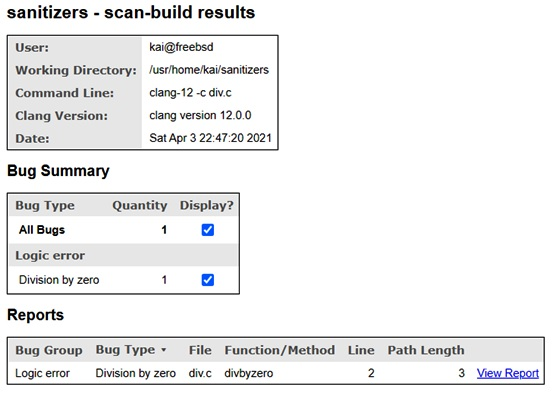
\includegraphics[width=0.6\textwidth]{content/3/chapter11/images/3.jpg}\\
图11.3 – 摘要页面
\end{center}

对于每个错误,摘要页面显示错误的类型、源中的位置,以及分析器找到错误的路径长度。提供了指向错误详细报告的链接。\par

下面的截图显示了错误的详细报告:\par


\hspace*{\fill} \par %插入空行
\begin{center}
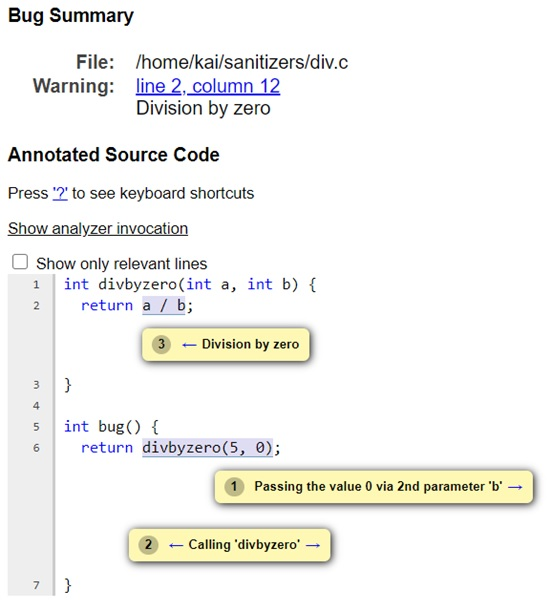
\includegraphics[width=0.6\textwidth]{content/3/chapter11/images/4.jpg}\\
图11.4 – 详细报告
\end{center}

有了详细的报告,就能够通过跟踪编号的气泡来验证错误。我们的示例中,以三个步骤展示了如何将0作为参数值传递导致除0错误。\par
 
确认工作需要人工进行。如果派生的约束对于某个检查器来说不够精确,那么可能会出现误报。也就是说,对于完全正确的代码会报告错误。根据这份报告,可以通过人工来确定假阳性。\par

您不限于该工具提供的检查器,还可以添加新的检查器。下一节将展示如何做到这一点。\par


\hspace*{\fill} \par %插入空行
\textbf{向Clang静态分析器添加新检查器}

要向Clang Static Analyzer添加一个新的检查器,需要创建一个checker类的新子类。静态分析程序尝试代码中所有可能的路径。分析器引擎在某些点生成事件,例如:在函数调用之前或之后。如果需要处理这些事件,则类必须为它们提供回调。Checker类和事件的注册在clang/include/clang/Stat\allowbreak icAnalyzer/Core/Checker.h头文件中提供。\par

通常,检查器需要跟踪一些符号。但是检查器不能管理状态,因为它不知道分析器引擎当前尝试的代码路径。因此,跟踪的状态必须在引擎中注册,并且只能用于ProgramStateRef实例。\par

许多库提供了必须成对使用的函数,例如:C标准库提供了malloc()和free()函数。由malloc()函数分配的内存必须由free()函数精确地释放一次。没有调用free()函数,或者多次调用它,是一个编程错误。这种编码模式还有很多实例,静态分析器为其中一些提供了检查器。\par

iconv库提供了将文本从一种编码转换为另一种编码的函数,例如:从Latin-1编码转换为UTF-16编码。要执行转换,实现需要分配内存。为了透明地管理内部资源,iconv库提供了iconv\underline{~}open()和iconv\underline{~}close()函数,它们必须成对使用。您可以实现一个检查器来进行检查。\par

为了检测错误,检查器需要跟踪从iconv\underline{~}open()函数返回的描述符。分析引擎为iconv\underline{~}open()函数的返回值返回一个SymbolRef实例。我们将这个符号与一个状态关联起来,以反映是否调用了iconv\underline{~}close()。对于状态,创建了IconvState类,其中只封装了一个bool值。\par

新IconvChecker类需要处理的四个事件:\par

\begin{itemize}
\item PostCall,发生在函数调用之后。调用iconv\underline{~}open()函数后,检索返回值的符号,并将其视为打开状态。

\item PreCall,发生在函数调用之前。在调用iconv\underline{~}close()函数之前,检查描述符的符号是否处于打开状态。如果不是,则说明描述符已经调用了iconv\underline{~}close()函数,并且检测到对该函数的双重调用。

\item DeadSymbol,当未使用的符号清除时发生。我们检查描述符的未使用符号是否仍处于打开状态。如果是,则检测到对iconv\underline{~}close()的未调用,这是一个资源泄漏。

\item PointerEscape,当分析器不能再跟踪符号时调用时,我们从状态中删除了符号,因为不能再推断描述符是否关闭了。

\end{itemize}

新的检查器在Clang项目中实现。让我们从将新的检查器添加到所有检查器集合开始,即clang/include/clang/StaticAnalyzer/Checkers/Checkers.td文件。每个检查器都与包相关联,我们的新检查器正在开发中,因此它属于alpha包。iconv API是posix标准化的API,所以它也属于unix包。在Checkers.td文件中找到UnixAlpha部分,并添加以下代码注册新的IconvChecker:\par

\begin{lstlisting}[caption={}]
def IconvChecker : Checker<"Iconv">,
	HelpText<"Check handling of iconv functions">,
	Documentation<NotDocumented>;
\end{lstlisting}

这将把新的检查器添加到已知检查器集合中,为命令行选项设置帮助文本,并声明没有关于此检查器的文档。\par

接下来,在clang/lib/StaticAnalyzer/Checkers/IconvChecker.cpp文件中实现检查器:\par

\begin{enumerate}
\item 为了实现,我们需要包含几个头文件。注册检查器需要BuiltinCheckerRegistration.h文件。Checker.h文件提供了Checker类的声明和事件的回调。CallEvent.h文件声明用于调用事件的类,CheckerContext类的声明需要CheckerContext.h文件,CheckerContext类是提供访问分析器状态的中心类:
\begin{lstlisting}[caption={}]
#include "clang/StaticAnalyzer/Checkers/
BuiltinCheckerRegistration.h"
#include "clang/StaticAnalyzer/Core/Checker.h"
#include "clang/StaticAnalyzer/Core/
PathSensitive/CallEvent.h"
#include "clang/StaticAnalyzer/Core/PathSensitive/
CheckerContext.h"
\end{lstlisting}

\item 为了避免输入命名空间名称:
\begin{lstlisting}[caption={}]
using namespace clang;
using namespace ento;
\end{lstlisting}

\item 我们将状态与代表iconv描述符的每个符号关联起来。状态可以是打开的,也可以是关闭的,我们使用了一个boolean类型的变量,该变量的真值表示打开状态。状态值封装在IconvState结构体中。此结构与FoldingSet数据结构一起使用,后者是过滤重复条目的散列表。为了使用这个数据结构实现,这里添加了Profile()方法,它设置这个结构的唯一位。我们将结构体放入一个匿名命名空间,以避免对全局命名空间的污染:
\begin{lstlisting}[caption={}]
namespace {
struct IconvState {
	const bool IsOpen;
	public:
	IconvState(bool IsOpen) : IsOpen(IsOpen) {}
	bool isOpen() const { return IsOpen; }
	bool operator==(const IconvState &O) const {
		return IsOpen == O.IsOpen;
	}
	void Profile(llvm::FoldingSetNodeID &ID) const {
		ID.AddInteger(IsOpen);
	}
};
}
\end{lstlisting}

\item IconvState结构体表示iconv描述符的状态,该描述符由SymbolRef类的符号表示。这最好使用映射来完成,将符号作为键,将状态作为值。如前所述,检查器不能保持状态。相反,状态必须注册到全局程序状态,这是通过REGISTER\underline{~}MAP\underline{~} with\underline{~}PROGRAMSTATE宏完成的。这个宏引入了IconvStateMap名称,我们稍后将使用它来访问映射:
\begin{lstlisting}[caption={}]
REGISTER_MAP_WITH_PROGRAMSTATE(IconvStateMap, SymbolRef,
							   IconvState)
\end{lstlisting}

\item 我们还在匿名命名空间中实现了IconvChecker类。请求的PostCall、PreCall、DeadSymbols和PointerEscape事件是Checker基类的模板参数:
\begin{lstlisting}[caption={}]
namespace {
	class IconvChecker
		: public Checker<check::PostCall, check::PreCall,
						 check::DeadSymbols,
						 check::PointerEscape> {
\end{lstlisting}

\item IconvChecker类只有CallDescription类型的字段,用于识别程序中iconv\underline{~}open()、iconv()和iconv\underline{~}close()函数调用:
\begin{lstlisting}[caption={}]
	CallDescription IconvOpenFn, IconvFn, IconvCloseFn;
\end{lstlisting}

\item report()的作用是:生成错误报告。该方法的重要参数是符号数组、错误类型和错误描述。该方法中,为每个符号创建一个错误报告,并将该符号标记为该错误感兴趣的符号。如果源范围作为参数提供,将添加到报表中。最后,生成报告:
\begin{lstlisting}[caption={}]
	void
	report(ArrayRef<SymbolRef> Syms, const BugType &Bug,
		   StringRef Desc, CheckerContext &C,
		   ExplodedNode *ErrNode,
		   Optional<SourceRange> Range = None) const {
		for (SymbolRef Sym : Syms) {
			auto R = std::make_unique
					<PathSensitiveBugReport>(
				Bug, Desc, ErrNode);
			R->markInteresting(Sym);
			if (Range)
				R->addRange(*Range);
			C.emitReport(std::move(R));
		}
	}
\end{lstlisting}

\item IconvChecker类的构造函数只使用函数名初始化CallDescription字段:
\begin{lstlisting}[caption={}]
public:
	IconvChecker()
		: IconvOpenFn("iconv_open"), IconvFn("iconv"),
			IconvCloseFn("iconv_close", 1) {}
\end{lstlisting}

\item checkPostCall()在分析器执行函数调用后调用。如果执行的函数不是一个全局的C函数,并且没有命名为iconv\underline{~}open,那么就没有什么可做的了:
\begin{lstlisting}[caption={}]
	void checkPostCall(const CallEvent &Call,
					   CheckerContext &C) const {
		if (!Call.isGlobalCFunction() ||
			!Call.isCalled(IconvOpenFn))
			return;
\end{lstlisting}

\item 否则,将尝试以符号的形式获取函数的返回值。为了在全局程序状态中存储具有打开状态的符号,我们需要从CheckerContext实例中获取一个ProgramStateRef实例。状态是不可变的,所以将符号添加到状态会产生一个新的状态。通过调用addTransition()方法,分析器引擎会更新状态:
\begin{lstlisting}[caption={}]
	if (SymbolRef Handle =
				Call.getReturnValue().getAsSymbol()) {
			ProgramStateRef State = C.getState();
			State = State->set<IconvStateMap>(
				Handle, IconvState(true));
			C.addTransition(State);
		}
	}
\end{lstlisting}

\item 调用checkDeadSymbols()方法来清理未使用的符号。我们循环遍历我们跟踪的所有符号,并询问SymbolReaper实例当前的符号是否已死:\par
\begin{lstlisting}[caption={}]
	void checkDeadSymbols(SymbolReaper &SymReaper,
						  CheckerContext &C) const {
		ProgramStateRef State = C.getState();
		SmallVector<SymbolRef, 8> LeakedSyms;
		for (auto SymbolState :
				State->get<IconvStateMap>()) {
			SymbolRef Sym = SymbolState.first;
			IconvState &St = SymbolState.second;
			
			if (SymReaper.isDead(Sym)) {
\end{lstlisting}

\item 如果符号已死,那么需要检查状态。如果状态仍然是打开的,那么这是一个潜在的资源泄漏。有一个例外:iconv\underline{~}open()在出现错误时返回-1。如果分析器处于处理此错误的代码路径中,则假设资源泄漏是错误的,因为函数调用失败。我们尝试从ConstraintManager实例获取该符号的值,如果该值为-1,则不认为该符号存在资源泄漏。向SmallVector实例添加一个泄漏的符号,以便稍后生成错误报告。最后,我们将死符号从程序状态中移除:
\begin{lstlisting}[caption={}]
				if (St.isOpen()) {
					bool IsLeaked = true;
					if (const llvm::APSInt *Val =
						State->getConstraintManager()
							.getSymVal(State, Sym))
						IsLeaked = Val->getExtValue() != -1;
					if (IsLeaked)
						LeakedSyms.push_back(Sym);
				}
			
				State = State->remove<IconvStateMap>(Sym);
			}
		}
\end{lstlisting}

\item 在循环之后,我们调用generateNonFatalErrorNode()方法。此方法转换到新的程序状态,如果此路径还没有错误节点,则返回一个错误节点。LeakedSyms容器保存泄漏符号的列表(可能为空),调用report()方法生成错误报告:
\begin{lstlisting}[caption={}]
		if (ExplodedNode *N =
				C.generateNonFatalErrorNode(State)) {
			BugType LeakBugType(this, "Resource Leak",
								"iconv API Error", true);
			report(LeakedSyms, LeakBugType,
				   "Opened iconv descriptor not closed", C,
					N);
		}
	}
\end{lstlisting}

\item 当分析器检测到无法跟踪参数的函数调用时,将调用checkPointerEscape()函数。这种情况下,必须假设不知道函数内部是否关闭了iconv描述符。唯一的例外是调用iconv()函数,该函数执行转换,并且已知不调用iconv\underline{~}close()函数。这就完成了IconvChecker类的实现:
\begin{lstlisting}[caption={}]
	ProgramStateRef
	checkPointerEscape(ProgramStateRef State,
						const InvalidatedSymbols &Escaped,
						const CallEvent *Call,
						PointerEscapeKind Kind) const {
		if (Kind == PSK_DirectEscapeOnCall &&
			Call->isCalled(IconvFn))
			return State;
		for (SymbolRef Sym : Escaped)
			State = State->remove<IconvStateMap>(Sym);
		return State;
	}
};
}
\end{lstlisting}

\item 最后,需要在CheckerManager实例上注册新的检查器。shouldRegisterIconvChecker()方法返回true,表示默认情况下应该注册IconvChecker, registerIconvChecker()方法执行注册。这两个方法都是通过Checkers.td文件生成的代码调用:
\begin{lstlisting}[caption={}]
void ento::registerIconvChecker(CheckerManager &Mgr) {
	Mgr.registerChecker<IconvChecker>();
}

bool ento::shouldRegisterIconvChecker(
const CheckerManager &Mgr) {
	return true;
}
\end{lstlisting}

\end{enumerate}

这就完成了新检查器的实现。只需要将文件名添加到clang/lib/StaticAnalyzer/Checkers/\par CmakeLists.txt文件中的源文件名列表中:\par

\begin{tcolorbox}[colback=white,colframe=black]
add\underline{~}clang\underline{~}library(clangStaticAnalyzerCheckers \\
… \\
\hspace*{0.5cm}IconvChecker.cpp \\
…)
\end{tcolorbox}

要编译新的检查器,要切换到build目录,并运行ninja命令:\par

\begin{tcolorbox}[colback=white,colframe=black]
\$ ninja
\end{tcolorbox}

可以使用保存在conf.c文件中的以下源代码测试新的检查器,该文件有两次对iconv\underline{~}close()函数的调用:\par

\begin{lstlisting}[caption={}]
#include <iconv.h>

void doconv() {
	iconv_t id = iconv_open("Latin1", "UTF-16");
	iconv_close(id);
	iconv_close(id);
}
\end{lstlisting}

学习了如何使用自己的检查器扩展Clang静态分析器,就可以使用这些知识来创建新的通用检查器,或将它们贡献给社区,或可以创建专门为您的需求构建的检查器,以提高自己产品的质量。 \par

静态分析器是利用Clang基础设施构建的,下一节将介绍如何使用自己的插件来扩展Clang。\par















